\documentclass{article}

\usepackage[english]{babel}
\usepackage[utf8]{inputenc}
\usepackage[]{hyperref}
\usepackage{graphicx, float}
\usepackage{subfig}
\usepackage{amssymb, amsmath, amsthm, stmaryrd}

%%%%%%%%%%%%%%%% Lengths %%%%%%%%%%%%%%%%
\setlength{\textwidth}{15.5cm}
\setlength{\evensidemargin}{0.5cm}
\setlength{\oddsidemargin}{0.5cm}

%%%%%%%%%%%%%%%% Variables %%%%%%%%%%%%%%%%
\def\projet{5}
\def\titre{Interpolation and Integration Methods}
\def\groupe{4}
\def\equipe{3}
\def\responsible{}
\def\secretary{}
\def\others{}

\begin{document}

%%%%%%%%%%%%%%%% Header %%%%%%%%%%%%%%%%
\begin{titlepage}
	\begin{center}
		\vspace*{1cm}
		\begin{figure}[htbp]
			%\centerline{\includegraphics[scale=0.5]{res/school-logo.jpg}}
		\end{figure}

		\vspace*{1.5cm}
		\rule{\linewidth}{1mm}\newline
		
		\textbf{\huge{Computer Science Project (n°5)}}
 
		\vspace{0.4cm}
		\LARGE{Interpolation and Integration Methods}
		\rule{\linewidth}{1mm}
		\vspace{0.1cm}

		\Large
		\textbf{Group \groupe, Team \equipe}\\
		\vspace{0.5cm}
		\Large
		\begin{center}
			\begin{tabular}{|c|c|}
				\hline
				\textbf{Leader} \\
				\hline
				\textbf{Secretary}  \\
				\hline
				\textbf{Programmers} \\
				\hline
			\end{tabular}
		\end{center}
		
		\begin{center}
			\begin{tabular}{|c|c|}
				\hline
				\textbf{Supervisor} & Dr. X \\
				\hline
				\textbf{Editor} & Dr. Y \\
				\hline
			\end{tabular}
		\end{center}
		\vspace{0.7cm}
 
		\vfill
		Computer Science\\
		School X\\
		2022-2023 
	\end{center}
\end{titlepage}

%%%%%%%%%%%%%%%% Main part %%%%%%%%%%%%%%%%

% Notes
% State that we used this airfoil maybe ?
% https://m-selig.ae.illinois.edu/ads/afplots/goe05k.gif

\tableofcontents

\section*{Introduction}

This report is composed of two preliminary parts: the first about interpolation methods and the second about integration methods.
\medbreak
The first part deals with the Cubic Spline interpolation method, which enables us to interpolate a function using a set of points.
This method is applied to a set of points of the goe05k airfoil, in order to obtain a smooth curve, which will be used in the third part.
\medbreak
The second part deals with the integration of a function, comparing the trapezoidal rule, the Simpson rule, the Romberg method, as well as the epsilon-integration method.
\medbreak
To conclude, the last part consists in applying the previous methods on an airfoil to obtain a pressure map around it, as well as the trajectories of air particles around it.


\section{Interpolation}

To analyse an airfoil's surface, a method to model it
with a function was necessary. As the UIUC Applied Aerodynamics Group's airfoil database only gives some pointson the surface, interpolation was needed. There are multiple interpolation
methods like Linear Interpolation or Cubic Spline Interpolation or even some fancier ones, but the selected method had to satisfy two requirements: be continuous and easily derivable.
The Cubic Spline interpolation method was used as it yields a continuous function, is easily derivable without adding algorithmic complexity and 
easy to implement.

\subsection{Cubic Spline Algorithm} \label{Cubic Spline algorithm}
The Cubic Spline approximation can be defined by equation~\ref{eq:cubic_spline_equation},
with $h_i = x_{i+1} - x_i$, $A_i(x) = \frac{x_{i+1}-x}{h_i}$ and $B_i(x) = \frac{x-x_i}{h_i}$:
\begin{equation}
	\label{eq:cubic_spline_equation}
	\begin{split}
		\omega_{\llbracket x_i;x_{i+1} \rrbracket}(x) = &A_i(x)y_i+B_i(x)y_{i+1} \\
		& + \frac{h_i^2}{6}\left(y_i^{''}\left(A_i^3(x) - A_i(x)\right)
		+ y_{i+1}^{''}\left(B_i^3(x) - B_i(x)\right)\right)
	\end{split}
\end{equation}
Each segment from $x_{i}$ to $x_{i+1}$ is interpolated with a cubic polynomial. This allows derivatives up to the second order.

To compute the derivative of a Cubic Spline interpolation, $\omega_i$ has to be derived. Its derivative is defined in equation~\ref{eq:derivative_cubic_spline}:
\begin{equation}
	\label{eq:derivative_cubic_spline}
	\omega_i^{'}(x) = \frac{y_{i+1} - y_i}{h_i} 
		+ \frac{h_i}{6}\left(
			y_i^{''}\left(1-3A_i^2(x)\right)
			+ y_{i+1}^{''}\left(3B_i^2(x)-1\right)
		\right)
\end{equation}

To ensure equation~\ref{eq:derivative_cubic_spline} can be derived, the following condition has to be met: $\forall i \in \llbracket 1;n \rrbracket~\omega_{i-1}^{'}(x_i) = \omega_i^{'}(x_i)$.
This condition can be modelled with equation~\ref{eq:equation_system_cubic_spline}:
\begin{equation}
	\label{eq:equation_system_cubic_spline}
	\frac{h_{i-1}}{6}y_{i-1}^{''} + \frac{h_{i-1} + h_i}{3}y_i^{''} + \frac{h_i}{6}y_{i+1}^{''}
	= \frac{y_{i+1}-y_i}{h_i}-\frac{y_i-y_{i-1}}{h_{i-1}}
\end{equation}
It is essential to specify the value of $y_0^{''}$ and $y_{n+1}^{''}$. For the rest of the experiments, the \textit{natural spline} method was used. It sets both $y_0^{''}$ and $y_{n+1}^{''}$ to $0$.

To get a single function that returns the correct $\omega_i(x)$ for a given $x$ in $\llbracket x_0; x_n \rrbracket$, a function $range(x)$ that searched for the correct range $\llbracket x_i;x_{i+1} \rrbracket$ for a given $x$ was implemented using a binary search algorithm for efficiency's sake as the list of $x_i$ is in increasing order.
Now, the function $\omega(x)$ that gives the interpolation function for all $x$ in $\llbracket x_0;x_n \rrbracket$ is defined as $\omega(x) = \omega_{range(x)}(x)$.

To check whether the Cubic Spline implementation was correctly implemented or not, the results were compared with those from a state of the art library for Cubic Spline interpolation: \verb|scipy|.
The results differed from \verb|scipy|'s one by an order of $10^{-18}$ which was acceptable.

\subsection{Interpolation of the goe05k Airfoil}
An airflow can be separated into 2 surfaces: the extrados (upper curves) and intrados (lower curves).
The database only gives points across both curves as seen in Figure~\ref{fig:sampled_goe05k_airfoil}

Therefore, the Cubic Spline interpolation method was used to model each part of the airfoil as a function to make the analysis of the airfoil possible, as seen in Figure~\ref{fig:interpolated_goe05k_airfoil}.

\begin{figure}[H]
	\centering
	\subfloat[\label{fig:sampled_goe05k_airfoil}\centering The Sampled points of the goe05k airfoil.]{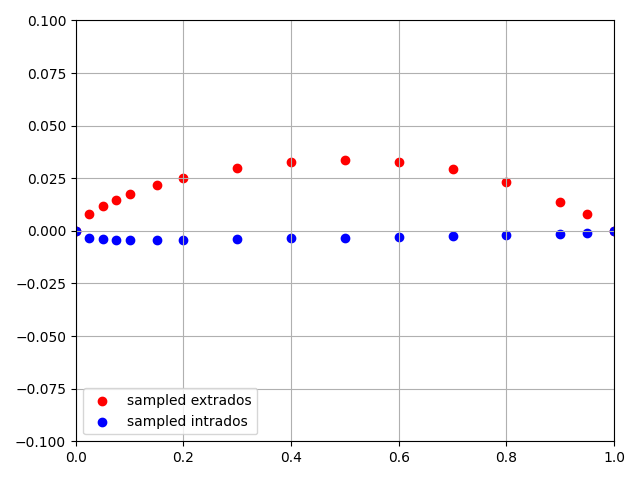
\includegraphics[width=0.45\linewidth]{res/goe05k_sampled.png}}
	\qquad
	\subfloat[\label{fig:interpolated_goe05k_airfoil}\centering The Interpolated goe05k airfoil.]{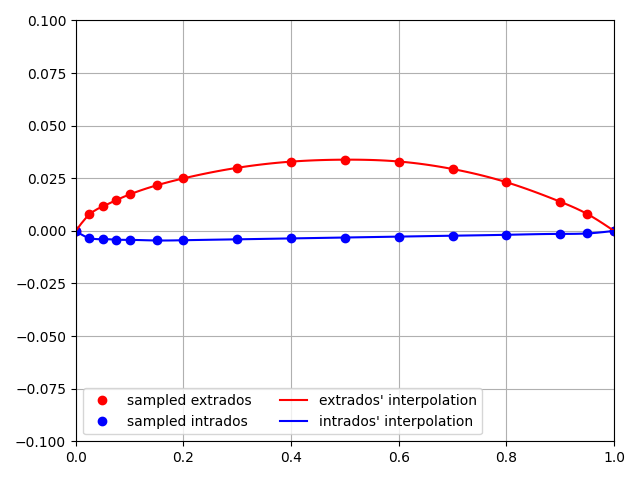
\includegraphics[width=0.45\linewidth]{res/goe05k_interpolated.png}}
	\caption{Interpolation of the goe05k airfoil.}
\end{figure}

\vspace*{-0.7cm}
\label{sec1}

\section{Integration }

In order to approximate the pressure on either side of the airfoil, an integral computation algorithm needs to be implemented.
Three different computation methods were considered, the goal being to find the algorithm with the highest convergence speed.


\subsection{Trapezoidal Method}

The trapezoidal method approximates the area under the curve of the function by dividing it into trapezoids and summing their areas.

Considering $n$ as the number of trapezoids used, the algorithm's time complexity is $\mathcal{O}(n)$.
By increasing $n$, the result's accuracy is improved, but the execution time is longer.

Despite its simplicity, the level of accuracy given by this method is very good for performing simple computations.


\subsection{Simpson's Rule}

Simpson's rule gives a second-order approximation of the integral of $f$ over $[a, b]$,
which means that the result is approximated using a parabola instead of a straight line, as in the previous method.
Its implementation uses an approximation similar to the one used in the previous method (see equation~\ref{eq:simpson-rule}).

\begin{equation}
	\label{eq:simpson-rule}
	\int_{x_i}^{x_{i + 1}} f(x) dx \approx \frac{x_{i + 1} - x_i}{3} \left[ f(x_i) + 4 \times f\left(\frac{x_i + x_{i + 1}}{2}\right) + f(x_{i + 1}) \right]
\end{equation}

Given this approximation, the integral of the function $f$ can be approximated by summing these results over all the sub-intervals,
$[x_i, x_{i + 1}]$ in $[a, b]$, as shown in equation~\ref{eq:simpson-rule-sum}.

\begin{equation}
	\label{eq:simpson-rule-sum}
	\int_a^b f(x) dx \approx \sum_{i = 0}^{n - 1} \int_{x_i}^{x_{i + 1}} f(x) dx
\end{equation}

As a result, this method's time complexity is $\mathcal{O}(n)$, where $n$ is the number of sub-intervals.


\subsection{Romberg's Method}

Romberg's method gives a more accurate approximation of the integral of $f$ over $[a, b]$ than the previous ones.
This method fills a table with the results of the trapezoidal method (first column), with a given number of evaluations.
The results of the previous rows are then used to compute the next rows, 
using both equations~\ref{eq:romberg-method-init} and~\ref{eq:romberg-method}.

It can be noted that the different rows represent integration methods using polynomials of increasing order.
Thus, this method generalizes the ones that were implemented before, considering both previous methods are special cases of this one, mathematically speaking.

\begin{equation}
	\label{eq:romberg-method-init}
	R_{n, 0} = h_n \times \left(\frac{f(a) + f(b)}{2} + \sum_{k = 0}^{2^{n - 1} - 1} f(x_k)\right)
	\text{where}\ h_n = \frac{b - a}{2^n}\ \text{and}\ x_k = a + k \times h_n
\end{equation}

\begin{equation}
	\label{eq:romberg-method}
	R_{n, m} = \frac{4^m R_{n, m - 1} - R_{n - 1, m - 1}}{4^m - 1}\ \text{where}\ n, m > 0
\end{equation}

In order to fill the table in the correct order, the columns must be filled from left to right, and the rows from top to bottom.
Once the table is filled, the result of the integral is the bottom right element of the table.

Another point to consider is that this method requires fewer evaluations on the function than the previous ones, given that evaluations are reused for the other columns.
Thus, when dealing with complex functions, this method is more efficient than the previous ones.

This method's time complexity depends on the table's size. In terms of memory, a 2-dimensional array is required. As a result, the memory complexity is $\mathcal{O}(n^2)$, where $n$ is the number of rows,
which means that this method requires more memory access, and thus slower.


\subsection{Integration with a Given Precision}

The following method offers the possibility of computing the integral of a function with a specific precision.
Its implementation uses the same algorithm from Romberg's method, except that it stops when the algorithm reaches the expected precision.

In fact, the algorithm stops when the equation $\left| R_{n, m} - R_{n - 1, m - 1} \right| \leq \epsilon$ is satisfied,
i.e. when the difference between the current result and the previous one is less than the given precision.

This method seemed to be the longest to apply, but is the most accurate among all the methods that were implemented, given that the precision can be chosen, which is essential for some applications.


\subsection{Comparison of Convergence Speeds}

The convergence speed of each method is displayed in Figure~\ref{fig:convergence}.

\medbreak

The trapezoidal method has a linear convergence rate, which means that the error decreases at a rate proportional to $1/n$, where $n$ is the number of sub-intervals.
This rate of convergence is not very fast, but it is generally sufficient for most applications.

\smallbreak
Simpson's rule has a faster convergence rate than the trapezoidal method, which is proportional to $1/n^2$.
This means that it typically requires fewer sub-intervals to achieve a given level of accuracy compared to the trapezoidal method. However, it can be sensitive to the shape of the function being integrated, and may not always be applicable.

\smallbreak
Romberg's method has a much faster convergence rate than both the trapezoidal method and Simpson's rule.
Its convergence rate is exponential, which means that the error decreases at a rate proportional to $2^{-2m}$, where $m$ is the number of iterations.
This means that it can achieve a high accuracy level with relatively few function evaluations, making it very efficient for many applications.
However, it requires more memory to store intermediate results, and can be more computationally intensive in some cases.

\smallbreak
Overall, the choice of integration method depends on the specific application and the desired level of accuracy.
The trapezoidal method is simple and robust, and is often a good choice for simple computations.
Simpson's rule is more accurate than the trapezoidal method, but may be less robust in some cases.
Romberg's method is the most accurate and efficient of the three, but requires more memory and computational resources.
Figure~\ref{fig:convergence} shows the convergence speed of each method.

\begin{figure}[htbp]
	\centering
	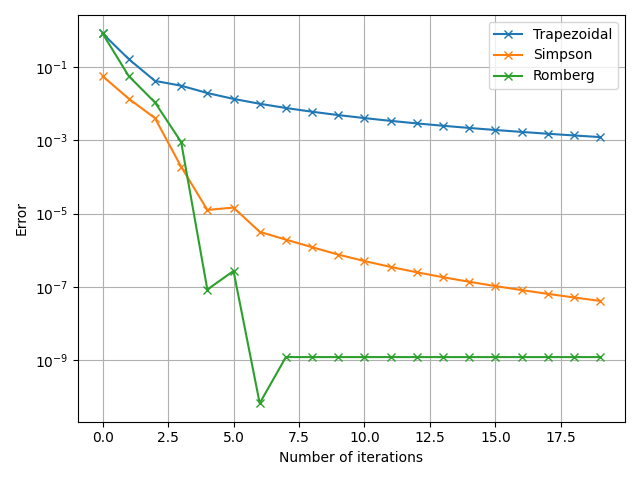
\includegraphics[width=0.45\linewidth]{res/convergence.png}
	\caption{Comparison of three different integration methods on $f(x) = \frac{1}{1 + x^2}$ over $[-1, 2]$.}
	\label{fig:convergence}
\end{figure}

\vspace*{-0.5cm}
\label{sec2}

\section{Application on an Airfoil}

The goal of this part was to use the previous functions to demonstrate the flow and behavior of
air around the airfoils of an airplane. In other words, showing how air moves around airfoils in order to produce that
lift force and as little air turbulence as possible. Moreover, the aim was to draw the pressure map that
the airfoils were going to be put under in order to deduce information like the maximum pressure
a wing can handle and which parts can handle more or less pressure.

\subsection{Modeling the Airflow }

An airfoil is supposed to operate in a laminar flow, which is a system where each air particle
moves along a curve that doesn't cross the path of another air particle, also known in physics 
as "\emph{no turbulence}". The closest particle to both surfaces moves exactly along the curves of an airfoil,
and the further the particle is, the flatter its path is. This can be summarized by saying that there is
\emph{no disturbance} in the supposed air system.


The goal was to be able to draw the trajectories of $N$ particles equally distributed in space. Many 
approximations were made in the field of fluid mechanics to simplify the movement equation and still 
be as accurate as possible. Let $h_{max}$ (i.e., $h_{min}$) be the maximum (i.e., minimum) height of the airfoil, 
$f$ be the function of the upper surface of the airfoil, $g$ be the function of the lower surface of the 
airfoil and $\lambda \in [0;1]$. The general formulas of the trajectory of any air particle above the upper 
surface and below the lower surface of the airfoil are respectively:

\begin{equation}
    \label{eq:airflow_up_low}
    f_\lambda(x) = (1-\lambda)f(x)+\lambda \times 3h_{max}\ \ \ \ \ \ \ \ 
    g_\lambda(x) = (1-\lambda)g(x)-\lambda \times 3h_{max}
\end{equation}

To draw the airflow for $N=30$ particles equally distributed in space, the first step was to draw the interpolation
of the airfoil, which was done in Figure~\ref{fig:interpolated_goe05k_airfoil}, using the cubic spline interpolation
 previously defined and described in section~\ref{Cubic Spline algorithm}.

The interval $[0;1]$ was separated into $15$ equal sections as $\lambda$ options like the following: $15$ particles
 above the upper surface and the rest under the lower surface using the equations above. This 
 application is illustrated by Figure \ref{fig:airflow}.

\begin{figure}[H]
\centering
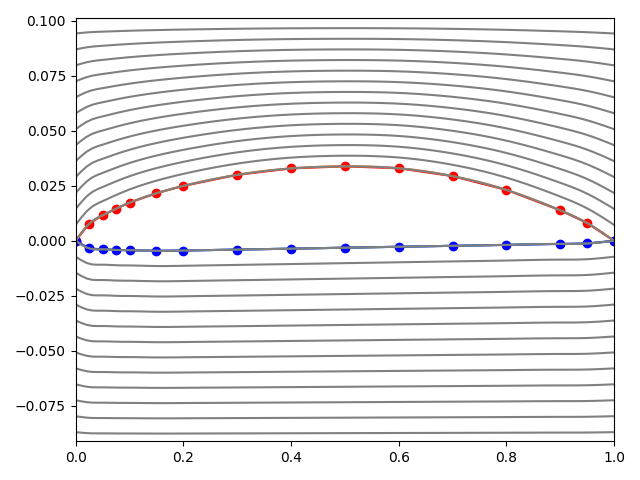
\includegraphics[width=0.5\linewidth]{res/air_flow.png}
\caption{The path of 30 particles in the space of an airfoil.}
\label{fig:airflow}
\end{figure}

In conclusion, the trajectories of air particles around the airfoil were succesfully drawn. The next step was to use these
trajectories to module the pressure map.

\subsection{Pressure Map }

All of the above amounts to plotting a pressure map around the wing, from which it is possible to deduce useful information about the airfoil's aerodynamic performance. Figure~\ref{fig:pressure_map} shows an example of pressure map.

\begin{figure}[H]
\centering
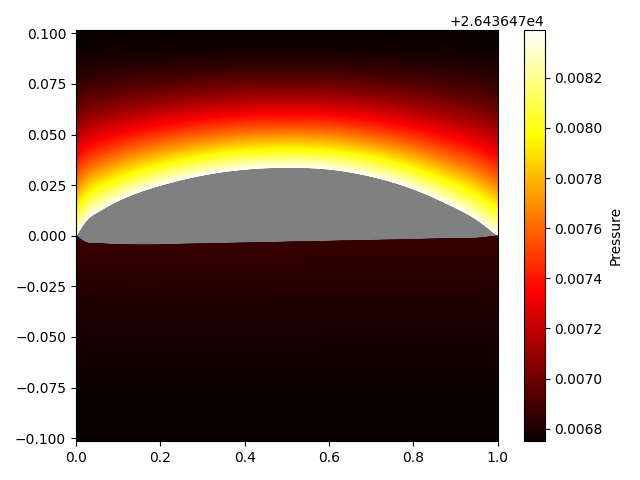
\includegraphics[width=0.5\linewidth]{res/pressure_map.png}
\caption{Pressure map example.}
\label{fig:pressure_map}
\end{figure}

The value of a pressure map lies in visually highlighting important information related to pressure around the airfoil being studied, processing it fluidly . It so appears that in the context of the mathematical modelisation chosen and the approximations made, air travels along a longer path right above the outer edge of the wing and decelerates at higher elevations, while air right below the inner edge of the wing seems to flow slower. Color coding facilitates the understanding of the map: darker areas express slower airflow rates, while lighter areas express faster airflow rates. The gray area corresponds to the wing itself, in which no flow naturally exists.

The function \verb|plot_pressure| generates the map by reading data from an input file, which contains the coordinates of the points tracing the airfoil's outer and inner edges. Cubic spline interpolation is then used to smooth out the wing's delimitations.

As described above, a parameter lambda is used to define the air particles flowing above and below the wing. For each of those, the airflow and line pressure are then calculated.

Finally, a pressure map such as Figure~\ref{fig:pressure_map} is ready to be plotted.
\label{sec3}

\end{document}